\documentclass[12pt]{article}
%%---------------------------------------------------------------------
% packages
% geometry
\usepackage{geometry}
% font
\usepackage{fontspec}
\defaultfontfeatures{Mapping=tex-text}  %%如果没有它,会有一些 tex 特殊字符无法正常使用,比如连字符。
\usepackage{xunicode,xltxtra}
\usepackage[BoldFont,SlantFont,CJKnumber,CJKchecksingle]{xeCJK}  % \CJKnumber{12345}: 一万二千三百四十五
\usepackage{CJKfntef}  %%实现对汉字加点、下划线等。
\usepackage{pifont}  % \ding{}
% math
\usepackage{amsmath,amsfonts,amssymb}
% color
\usepackage{color}
\usepackage{xcolor}
\definecolor{EYE}{RGB}{199,237,204}
\definecolor{FLY}{RGB}{128,0,128}
\definecolor{ZHY}{RGB}{139,0,255}
% graphics
\usepackage[americaninductors,europeanresistors]{circuitikz}
\usepackage{tikz}
\usetikzlibrary{positioning,arrows,shadows,shapes,calc,mindmap,trees,backgrounds}  % placements=positioning
\usepackage{graphicx}  % \includegraphics[]{}
\usepackage{subfigure}  %%图形或表格并排排列
% table
\usepackage{colortbl,dcolumn}  %% 彩色表格
\usepackage{multirow}
\usepackage{multicol}
\usepackage{booktabs}
% code
\usepackage{fancyvrb}
\usepackage{listings}
% title
\usepackage{titlesec}
% head/foot
\usepackage{fancyhdr}
% ref
\usepackage{hyperref}
% pagecolor
\usepackage[pagecolor={EYE}]{pagecolor}
% tightly-packed lists
\usepackage{mdwlist}

\usepackage{styles/iplouccfg}
\usepackage{styles/zhfontcfg}
\usepackage{styles/iplouclistings}

%%---------------------------------------------------------------------
% settings
% geometry
\geometry{left=2cm,right=1cm,top=2cm,bottom=2cm}  %设置 上、左、下、右 页边距
\linespread{1.5} %行间距
% font
\setCJKmainfont{Adobe Kaiti Std}
%\setmainfont[BoldFont=Adobe Garamond Pro Bold]{Apple Garamond}  % 英文字体
%\setmainfont[BoldFont=Adobe Garamond Pro Bold,SmallCapsFont=Apple Garamond,SmallCapsFeatures={Scale=0.7}]{Apple Garamond}  %%苹果字体没有SmallCaps
\setCJKmonofont{Adobe Fangsong Std}
% graphics
\graphicspath{{figures/}}
\tikzset{
    % Define standard arrow tip
    >=stealth',
    % Define style for boxes
    punkt/.style={
           rectangle,
           rounded corners,
           draw=black, very thick,
           text width=6.5em,
           minimum height=2em,
           text centered},
    % Define arrow style
    pil/.style={
           ->,
           thick,
           shorten <=2pt,
           shorten >=2pt,},
    % Define style for FlyZhyBall
    FlyZhyBall/.style={
      circle,
      minimum size=6mm,
      inner sep=0.5pt,
      ball color=red!50!blue,
      text=white,},
    % Define style for FlyZhyRectangle
    FlyZhyRectangle/.style={
      rectangle,
      rounded corners,
      minimum size=6mm,
      ball color=red!50!blue,
      text=white,},
    % Define style for zhyfly
    zhyfly/.style={
      rectangle,
      rounded corners,
      minimum size=6mm,
      ball color=red!25!blue,
      text=white,},
    % Define style for new rectangle
    nrectangle/.style={
      rectangle,
      draw=#1!50,
      fill=#1!20,
      minimum size=5mm,
      inner sep=0.1pt,}
}
\ctikzset{
  bipoles/length=.8cm
}
% code
\lstnewenvironment{VHDLcode}[1][]{%
  \lstset{
    basicstyle=\footnotesize\ttfamily\color{black},%
    columns=flexible,%
    framexleftmargin=.7mm,frame=shadowbox,%
    rulesepcolor=\color{blue},%
%    frame=single,%
    backgroundcolor=\color{yellow!20},%
    xleftmargin=1.2\fboxsep,%
    xrightmargin=.7\fboxsep,%
    numbers=left,numberstyle=\tiny\color{blue},%
    numberblanklines=false,numbersep=7pt,%
    language=VHDL%
    }\lstset{#1}}{}
\lstnewenvironment{VHDLmiddle}[1][]{%
  \lstset{
    basicstyle=\scriptsize\ttfamily\color{black},%
    columns=flexible,%
    framexleftmargin=.7mm,frame=shadowbox,%
    rulesepcolor=\color{blue},%
%    frame=single,%
    backgroundcolor=\color{yellow!20},%
    xleftmargin=1.2\fboxsep,%
    xrightmargin=.7\fboxsep,%
    numbers=left,numberstyle=\tiny\color{blue},%
    numberblanklines=false,numbersep=7pt,%
    language=VHDL%
    }\lstset{#1}}{}
\lstnewenvironment{VHDLsmall}[1][]{%
  \lstset{
    basicstyle=\tiny\ttfamily\color{black},%
    columns=flexible,%
    framexleftmargin=.7mm,frame=shadowbox,%
    rulesepcolor=\color{blue},%
%    frame=single,%
    backgroundcolor=\color{yellow!20},%
    xleftmargin=1.2\fboxsep,%
    xrightmargin=.7\fboxsep,%
    numbers=left,numberstyle=\tiny\color{blue},%
    numberblanklines=false,numbersep=7pt,%
    language=VHDL%
    }\lstset{#1}}{}
% pdf
\hypersetup{pdfpagemode=FullScreen,%
            pdfauthor={Haiyong Zheng},%
            pdftitle={Title},%
            CJKbookmarks=true,%
            bookmarksnumbered=true,%
            bookmarksopen=false,%
            plainpages=false,%
            colorlinks=true,%
            citecolor=green,%
            filecolor=magenta,%
            linkcolor=cyan,%red(default)
            urlcolor=cyan}
% section
%http://tex.stackexchange.com/questions/34288/how-to-place-a-shaded-box-around-a-section-label-and-name
\newcommand\titlebar{%
\tikz[baseline,trim left=3.1cm,trim right=3cm] {
    \fill [cyan!25] (2.5cm,-1ex) rectangle (\textwidth+3.1cm,2.5ex);
    \node [
        fill=cyan!60!white,
        anchor= base east,
        rounded rectangle,
        minimum height=3.5ex] at (3cm,0) {
        \textbf{\thesection.}
    };
}%
}
\titleformat{\section}{\Large\bf\color{blue}}{\titlebar}{0.1cm}{}
% head/foot
\setlength{\headheight}{15pt}
\pagestyle{fancy}
\fancyhf{}

\chead{\color{black!50!green}Assignment \#1}

\lfoot{\color{blue!50!green}Zhu Yafei}
\cfoot{\color{blue!50!green}\href{http://vision.ouc.edu.cn/~zhenghaiyong}{CVBIOUC}}
\rfoot{\color{blue!50!green}$\cdot$\ \thepage\ $\cdot$}
\renewcommand{\headrulewidth}{0.4pt}
\renewcommand{\footrulewidth}{0.4pt}

%%---------------------------------------------------------------------
\begin{document}
%%---------------------------------------------------------------------
%%---------------------------------------------------------------------
% \titlepage
\title{\vspace{-2em}CV2015Spring---Assignment \#\textbf{1}\\
\normalsize{Due: Apr 12, 2015 (10:00AM)}}
\author{Zhu Yafei}
\date{\vspace{-0.7em}March 26, 2015\vspace{-0.7em}}
%%---------------------------------------------------------------------
\maketitle\thispagestyle{fancy}
%%---------------------------------------------------------------------
\maketitle
%\tableofcontents 


%\section{Programming problem: salient object detection}
\section{Assignment requirement}

For this assignment, you will implement a version of the salient object detection technique. See Figure~\ref{fig: result} for an example.

\begin{figure}[!ht]
  \centering 
  \subfigure[]{ 
    \label{fig: result: a} %% label for first subfigure 
    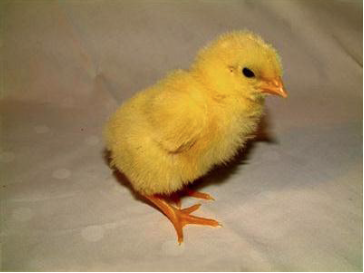
\includegraphics[width=0.3\textwidth]{OriginImage}} 
  \subfigure[]{ 
    \label{fig: result: b} %% label for second subfigure 
    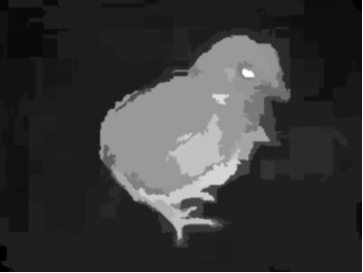
\includegraphics[width=0.3\textwidth]{SaliencyMap}} 
  \caption{Salient object detection.}
  \label{fig: result} %% label for entire figure 
\end{figure}

Your method must be region-based, and at least one feature and one prior should be used. I will give you some tips for the implementation in the following sections.

\section{Tips}

The whole framework of the implementation for salient object detection is shown in Figure~\ref{fig: framework}, it may serve as a reference for your assignment. Next, I will introduce the implementation and requirement of each part of the framework for you.

\begin{figure}[!ht]
\centering
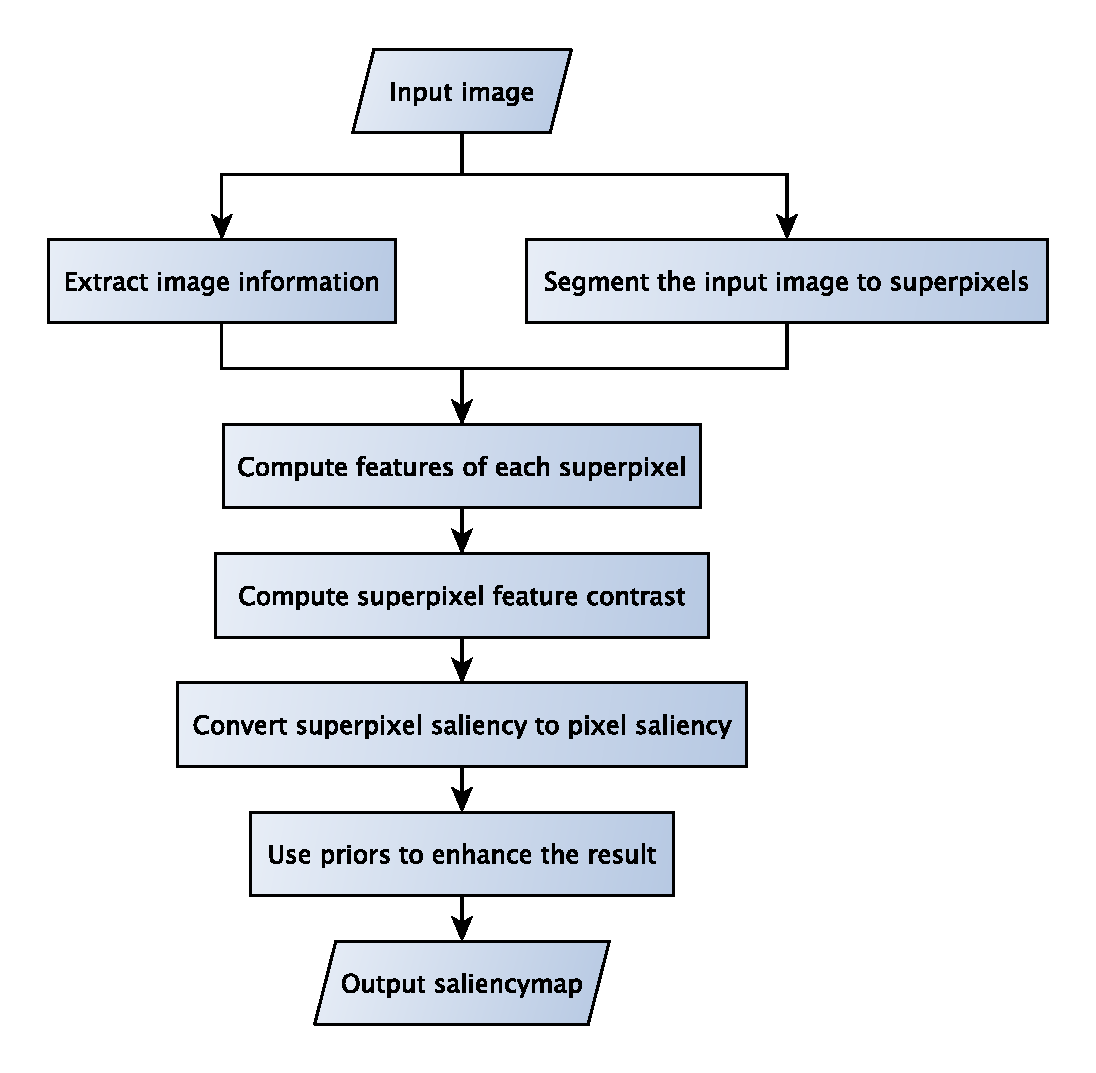
\includegraphics[width=0.6\textwidth]{framework.eps}
\caption{Framework of the implementation for salient object detection.}
\label{fig: framework}
\end{figure}

\subsection{Input image}

A simple dataset can be downloaded from the website\footnote{\url{http://research.microsoft.com/en-us/um/people/jiansun/SalientObject/salient_object.htm}}. Pick one or several images from the dataset randomly for test.

\subsection{Step 1-1: Extract image information (15 points)}

\begin{description}
\item[Input] The input color image ($m \times n \times 3$ matrix), $m$ is the width of the input image, $n$ is the height of the input image.
\item[Output] $m \times n$ matrix. 
\item[Implementation] This step determines the regional feature you want to use in step 2, and you have two choices (choose at least one feature for this assignment):
\begin{itemize}
\item Color information
\begin{itemize}
\item[-] You should quantize each color channel (RGB) to reduce the number of colors (such as from $256$ to $16$), then the number of color is reduced to $16 \times 16 \times 16 = 4096$. In order to create a bin for each color, you can use a number ($1 \sim 4096$) instead of (R, G, B) values to represent a color uniquely.
\end{itemize}
\item Texture information
\begin{itemize}
\item[-] You should compute the LBP value of each pixel here.  
\end{itemize}
\end{itemize}
\item[Hint] The extraction of color/texture information can refer to the matlab code from the website\footnote{\url{http://jianghz.com/projects/saliency_drfi/index.html}}, which also contains the computation of color histogram and texture histogram of superpixels in step 2 and the conversion of superpixel saliency to pixel saliency in step 4.
\end{description}

\subsection{Step 1-2: Segment the input image to superpixels (20 points)}

\begin{description}
\item[Input] The input color image ($m \times n \times 3$ matrix), $m$ is the width of the input image, $n$ is the length of the input image. 
\item[Output]  Superpixel segmentation matrix ($m \times n$ matrix), the value of the pixel in this matrix is just a label to indicate the superpixel it belongs to, and pixels of the same superpixel are labeled the same value. 
\item[Hint] There are a lot of superpixel segmentation algorithms, I recommend you to use SLIC\footnote{\url{http://www.vlfeat.org}}, which is fast and easy to implement.
\end{description}

\subsection{Step 2: Compute features of each superpixel (15 points)}

\begin{description}
\item[Input] Image information matrix, superpixel segmentation matrix. 
\item[Output] $h$ histograms, $h$ is the number of superpixels after segmentation.
\item[Implementation] The feature you choose here is based on the information you extracted in step 1-1:
\begin{itemize}
\item Compute color histogram feature of each superpixel, which means counting number of pixels for each color and store it in histogram's bins.
\item Compute texture histogram feature of each superpixel
\end{itemize}
\item[Hint] Useful function in matlab for histogram computation: \emph{hist}.
\end{description}

\subsection{Step 3: Compute superpixel feature contrast (20 points)}

\begin{description}
\item[Input] $h$ histograms.
\item[Output] $h$ values, each value indicates the global feature contrast of a superpixel.
\item[Instructions] Saliency can be defined as uniqueness in terms of local or global regional contrast. For simplicity, I recommend you to compute global regional contrast, which means that the saliency of a superpixel should be computed as its feature contrast of all the other superpixels in the image. 
\item[Theory] The formulation for histogram distance is as follows:
\begin{align}
\chi^2(\textbf{h}_1, \textbf{h}_2) = \sum_{i=1}^{b}\frac{2(h_{1i}-h_{2i})^2}{h_{1i}+h_{2i}}
\end{align}
where $\textbf{h}_1$ and $\textbf{h}_2$ are color histograms of two distinct regions,  $h_{1i}$ and $h_{2i}$ are the $i$th component of $\textbf{h}_1$ and $\textbf{h}_2$ respectively, $b$ is the number of histogram bins. Moreover, both histograms are normalized, i.e. their entries sum up to one.
\end{description}

\subsection{Step 4: Convert superpixel saliency to pixel saliency (15 points)}

\begin{description}
\item[Input] $h$ values, superpixel segmentation matrix.
\item[Output] An initial saliency map ($m \times n$ matrix).
\item[Implementation] Assign all the pixels of the same superpixel the same saliency value. 
\end{description}

\subsection{Step 5: Use priors to enhance the result (15 points)}

\begin{description}
\item[Input] Initial saliency map,.
\item[Output] Final saliency map.
\item[Implementation] Here you have two choices (choose at least one prior for this assignment):
\begin{itemize}
\item Center prior
\item Color prior
\end{itemize}
Multiply the initial saliency map with the prior you choose, you can obtain the final saliency map.
\item[Hint] You can download the source code from this website\footnote{\url{http://sse.tongji.edu.cn/linzhang/va/SDSP/SDSP.htm}} for reference.
\end{description}

\section{Submission instructions}

\subsection{What to hand in?}

\begin{itemize}
\item Your matlab code (Show your medial result in your code)
\item A report containing the following:
\begin{itemize}
\item Your name at the top
\item A brief explanation of your implementation strategy (in English)
\end{itemize}
\end{itemize}

\subsection{Where to hand in?}

Submit to Piazza in form of a followup below my assignment note.





%\bibliographystyle{plain}
%
%\bibliography{Assignment1} 

%%---------------------------------------------------------------------
\end{document}
